%%%%
\section{Meteorologia local e Harmatão}

Para melhor entendimento das fontes poluídoras, analisa-se a seguir a 
dinâmica de ventos a partir de dados da estação meteorológia do 
aeroporto de Acra (Kotoka International Airport) disponibilizados no site da 
National Oceanic and Atmospheric Administration - United States Department of 
Commerce (NOAA). As rosas dos ventos foram plotadas usando a biblioteca 
openair desenvolvida por \citet{carslaw2012}.

\begin{figure}[H]
  \centering
  \includegraphics[width=0.5\textwidth]{../outputs/windRose2007.pdf}
  \caption{Rosa do ventos para Acra/2007. \label{fg:rosaCompleta}}
\end{figure}

A figura \ref{fg:rosaCompleta} mostra a distribuição de frequência da direção 
dos ventos em conjunto como a intensidade para o ano de 2007, sendo que a direção 
predominante de origem dos ventos de superfície está no quadrante sudoeste.

Acra é uma região litorânea e na observação horária, média no período de 
amostragem, identifica-se pelo gráfico da figura \ref{fig:windRose_horaria}, 
que a direção e intensidade dos ventos apresentam forte componente regional, 
associável à brisa marinha.

A brisa marinha, de vento próximo da direção sul (oceano), começa a se formar a 
partir do amanhancer, enfraquecendo o vento oeste, que persistiu durante a noite,
e ganha mais intensidade particularmente a partir de 12h. Ganha intensidade e 
desloca-se à direção oeste na medida em que as horas avançam 
(deslocamento à direita do sentido do movimento - ação típica do efeito de 
Coriolis no hemisfério Norte). 
Verificamos ainda que durante o período noturno há maior incidência de calmaria
e intensidade de ventos mais fracas, enquanto durante o dia os ventos médios são
mais intensos, em função do ciclo de irradiação solar.

\begin{figure}[H]
  \centering
  \includegraphics[width=\linewidth]{../outputs/windRose_horaria.pdf}
  \caption{Rosa do ventos horária para Acra/2007. \label{fig:windRose_horaria}}
\end{figure}

Mensalmente, figura \ref{fig:windRose_mensal}, pode-se acompanhar o 
comportamento sazonal do vento. No Verão temos maior quantidade de radiação 
solar, fortalecendo a formação de brisa marinha e, consequentemente, havendo 
maior tempo para a velocidade do vento intensificar-se e para processar-se um 
deslocamento para oeste (Coriolis). 

Na maior parte do verão, Gana localiza-se, em termos de padrão global de 
circulação, no hemisfério sul, ou seja, abaixo da Zona de Convergência 
Intertropical (ZCIT). Neste período, as intensidades de vento são maiores e 
são menores as frequências de calmarias. No período do inverno, Gana 
posiciona-se a norte da ZCIT, e observa-se com isso maior incidência de 
ventos com origem neste hemisfério (veja-se particularmente o mês 
de janeiro), 
com velocidades médias do vento um pouco menores e maior percentual
de calmaria. É nesta época que Gana e o deserto do Saara situam-se no mesmo 
sistema de circulação global, ocorrendo o Harmatão. 

Nos meses de ocorrência do Harmatão (inverno), há um pequeno aumento da 
frequência de ventos de nordeste ao nível do solo (direção do Saara), mas a 
maior parte do particulado que este vento transporta passa por Gana em 
altitudes superiores \citep{breuning2005}, interferindo pouco no predomínio 
da brisa marinha na circulação local.%

\newpage
\begin{figure}[H]
  \centering
  \includegraphics[width=\linewidth]{../outputs/windRose_mensal.pdf}
  \caption{Rosa do ventos mensal para Acra/2007. \label{fig:windRose_mensal}}
\end{figure}

%%%%
\newpage
\subsection{Circulação Global}

Na rosa do ventos para o ano de 2007 (figura \ref{fg:rosaCompleta}) nota-se 
que praticamente não há ventos de norte e nordeste. Mesmo no inverno 
(figura \ref{fig:windRose_mensal}) quando Gana está no hemisfério norte em 
termos da circulação global, a frequência de ventos nordeste na superfície 
continua baixa. 
Como descrito por \citet{breuning2005}, o Harmatão é um vento nordeste 
que transporta areia do deserto do Saara a altas altitudes (1000 m).

Para contraste dos ventos médios em altas altidudes com os de superfície, 
dados de re-análise disponibilizados pela ECMWF de dezembro de 
2007 e janeiro de 2008 foram utilizados. Com recorte na longitude entre 2
0 oeste e 60 leste e latitude de 30 sul a 40 norte, selecionou-se assim o 
continente Africano e parte dos oceanos atlântico e índico. 
Os mapas da figura \label{fig:ECMWF10} mostram
ventos próximos a superfície e os da \label{fig:ECMWF1000} os ventos na altitude 
próxima a 1000 metros para o mesmo período. 
Na superfície, é possível notar o regime de brisa marinha, com entrada de vento 
do mar. Em 1000 metros, os ventos de nordeste são muitos mais intensos e 
frequentes que na superfície, caracterizando a presença do Harmatão. 

\begin{figure}[H]
  \centering
  \begin{subfigure}[b]{0.5\linewidth}
    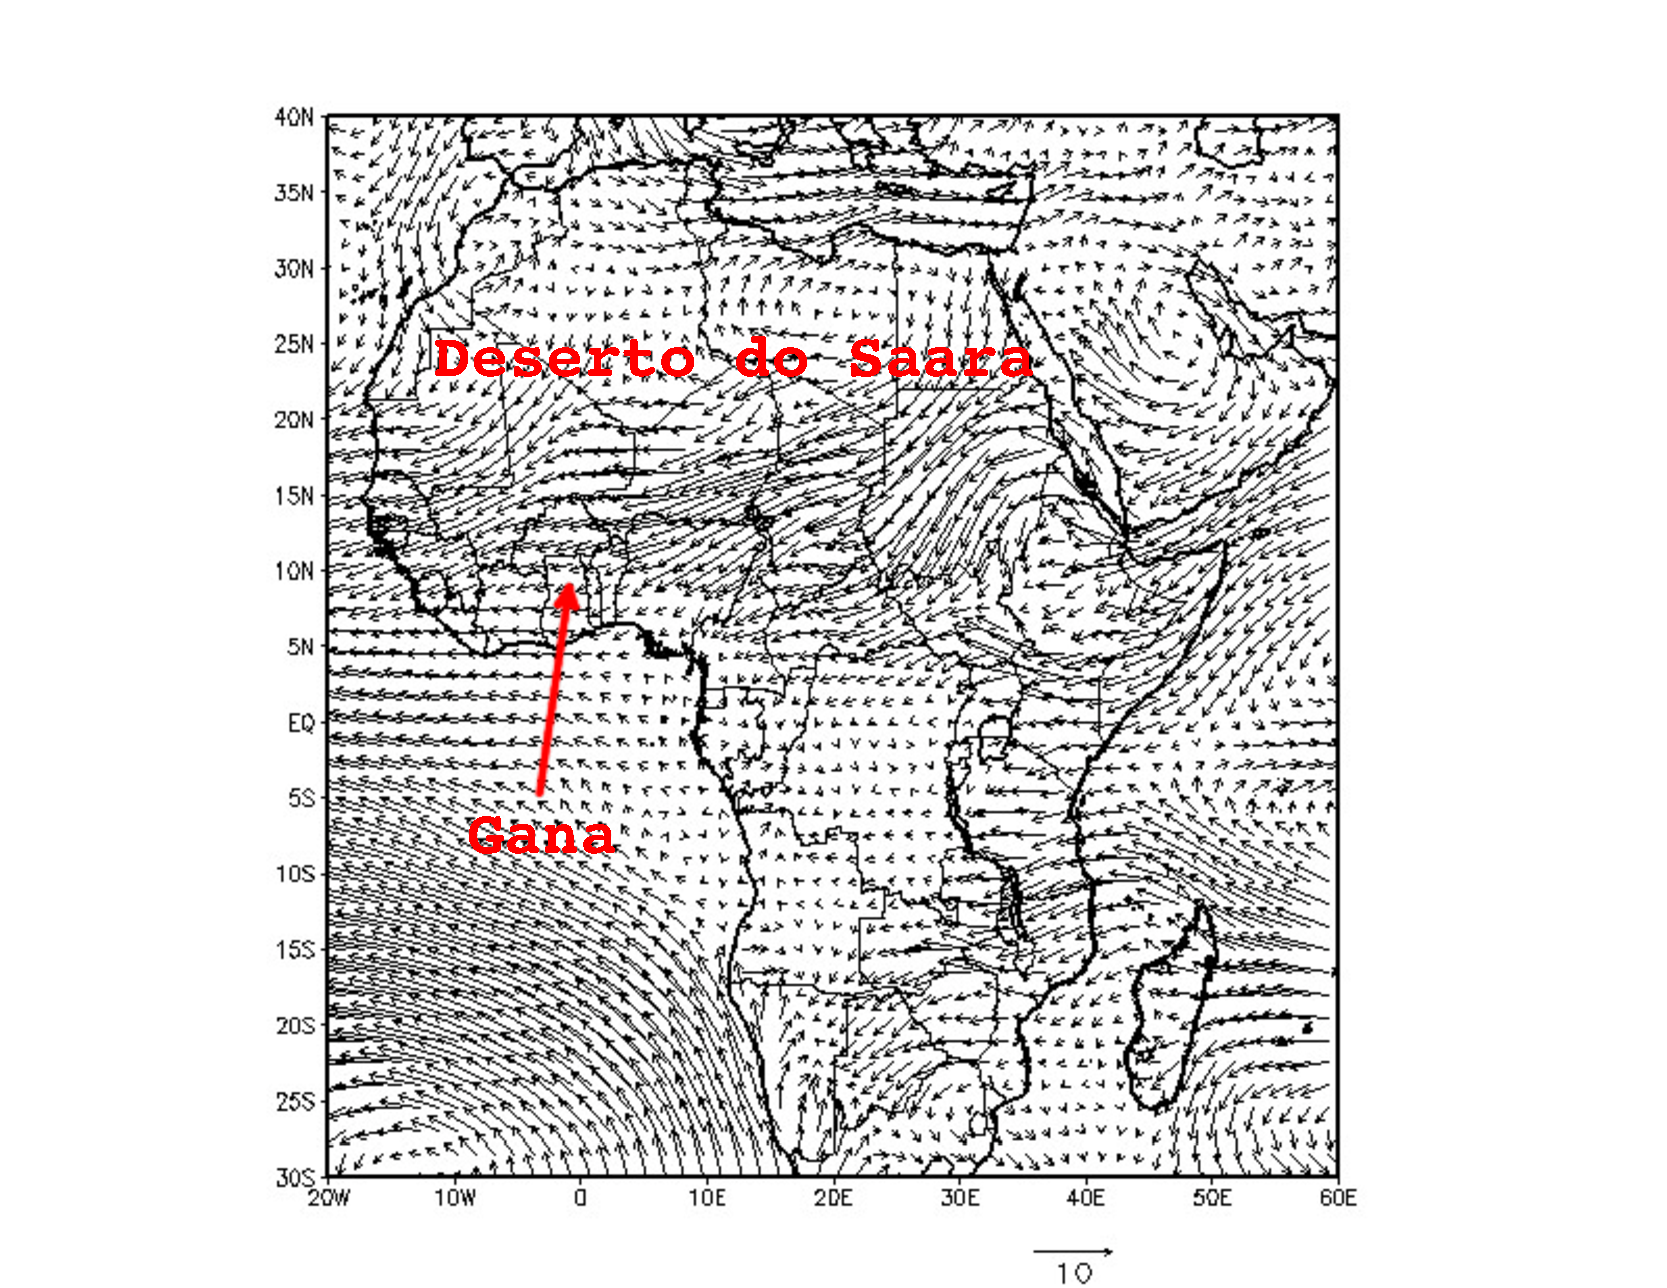
\includegraphics[width=\linewidth]{../inputs/grads/gimp/875hPa/DEZ_2007.pdf}
    \caption{Dezembro de 2007}
  \end{subfigure}%
%  \hspace{0.5cm}
  \begin{subfigure}[b]{0.5\linewidth}
    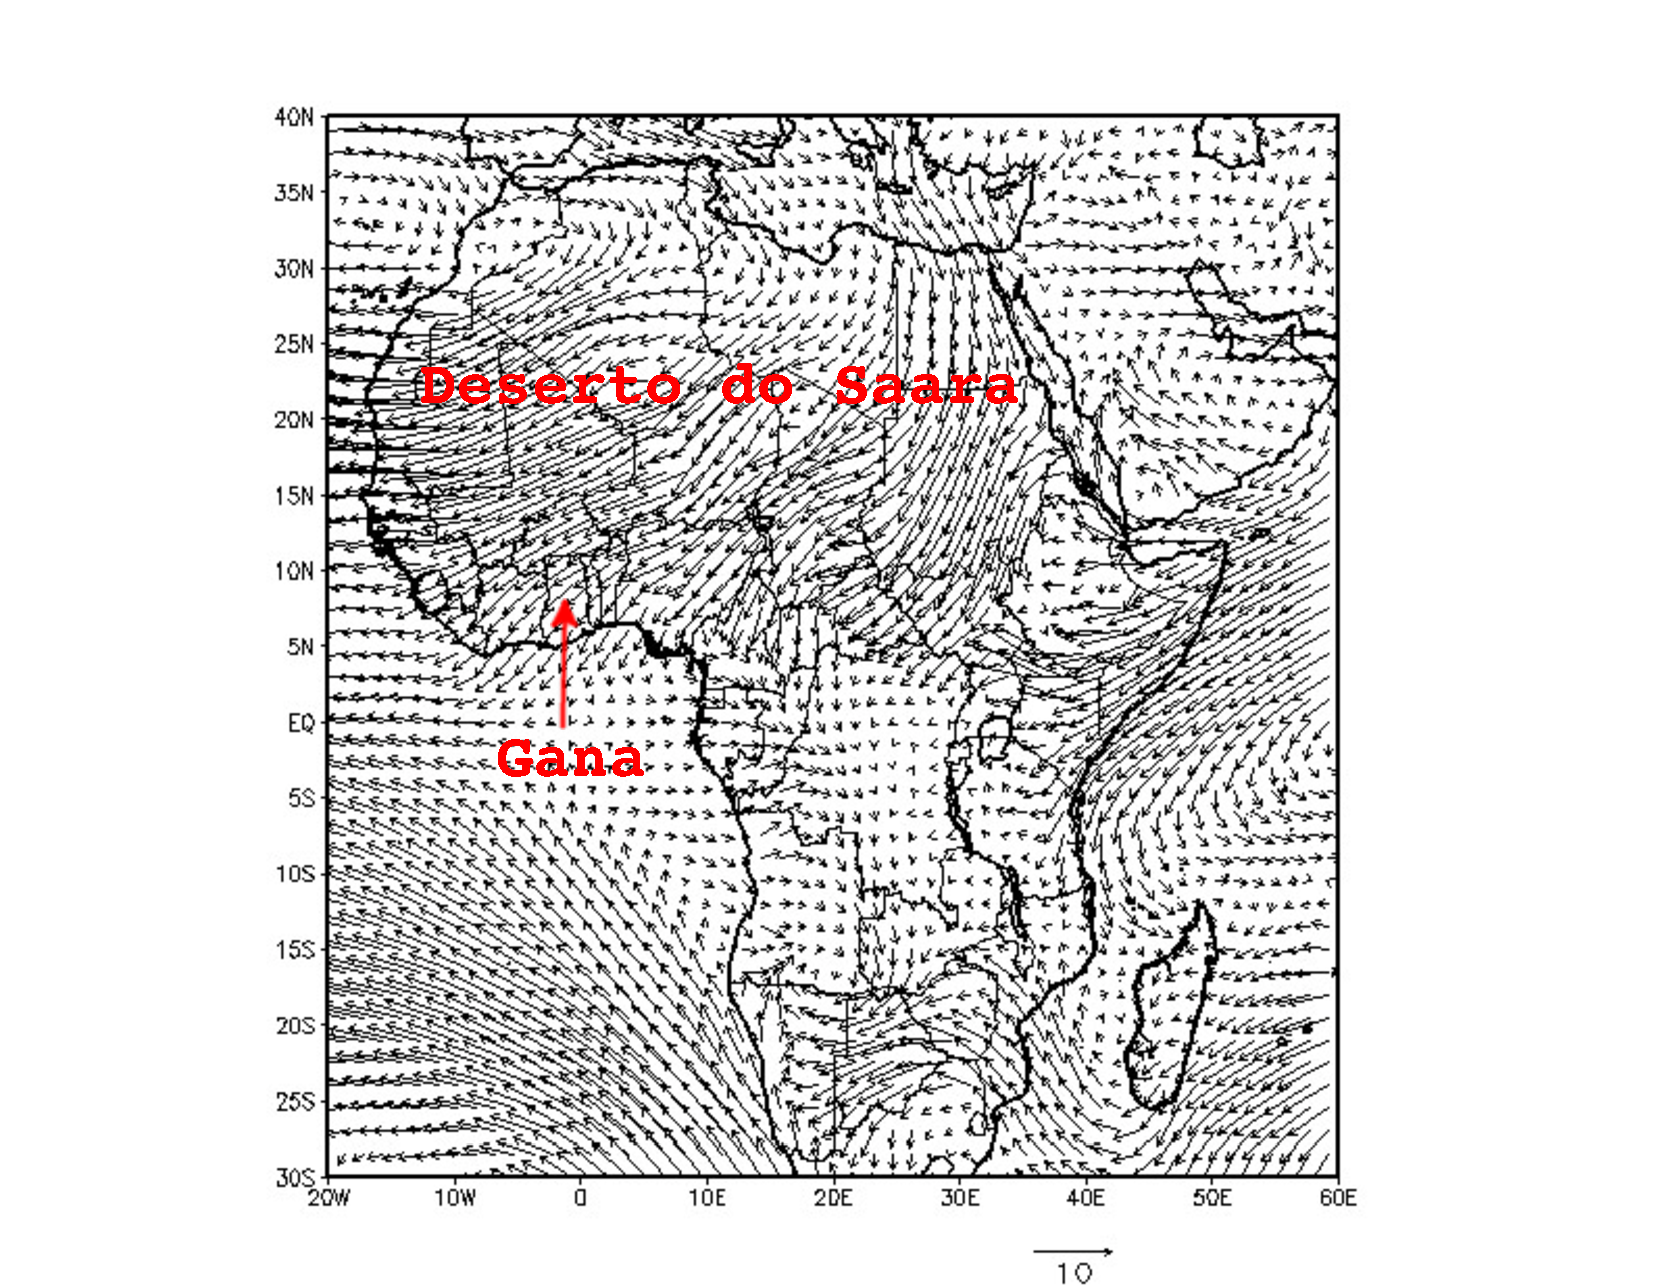
\includegraphics[width=\linewidth]{../inputs/grads/gimp/875hPa/JAN_2008.pdf}
    \caption{Janeiro de 2008}
  \end{subfigure}
  \caption{Intensidade e direção do vento médio na altitude de 1000 metros 
           sobre o continente Africano. \label{fig:ECMWF1000}}
\end{figure}

\begin{figure}[H]
  \centering
  \begin{subfigure}[b]{0.5\linewidth}
    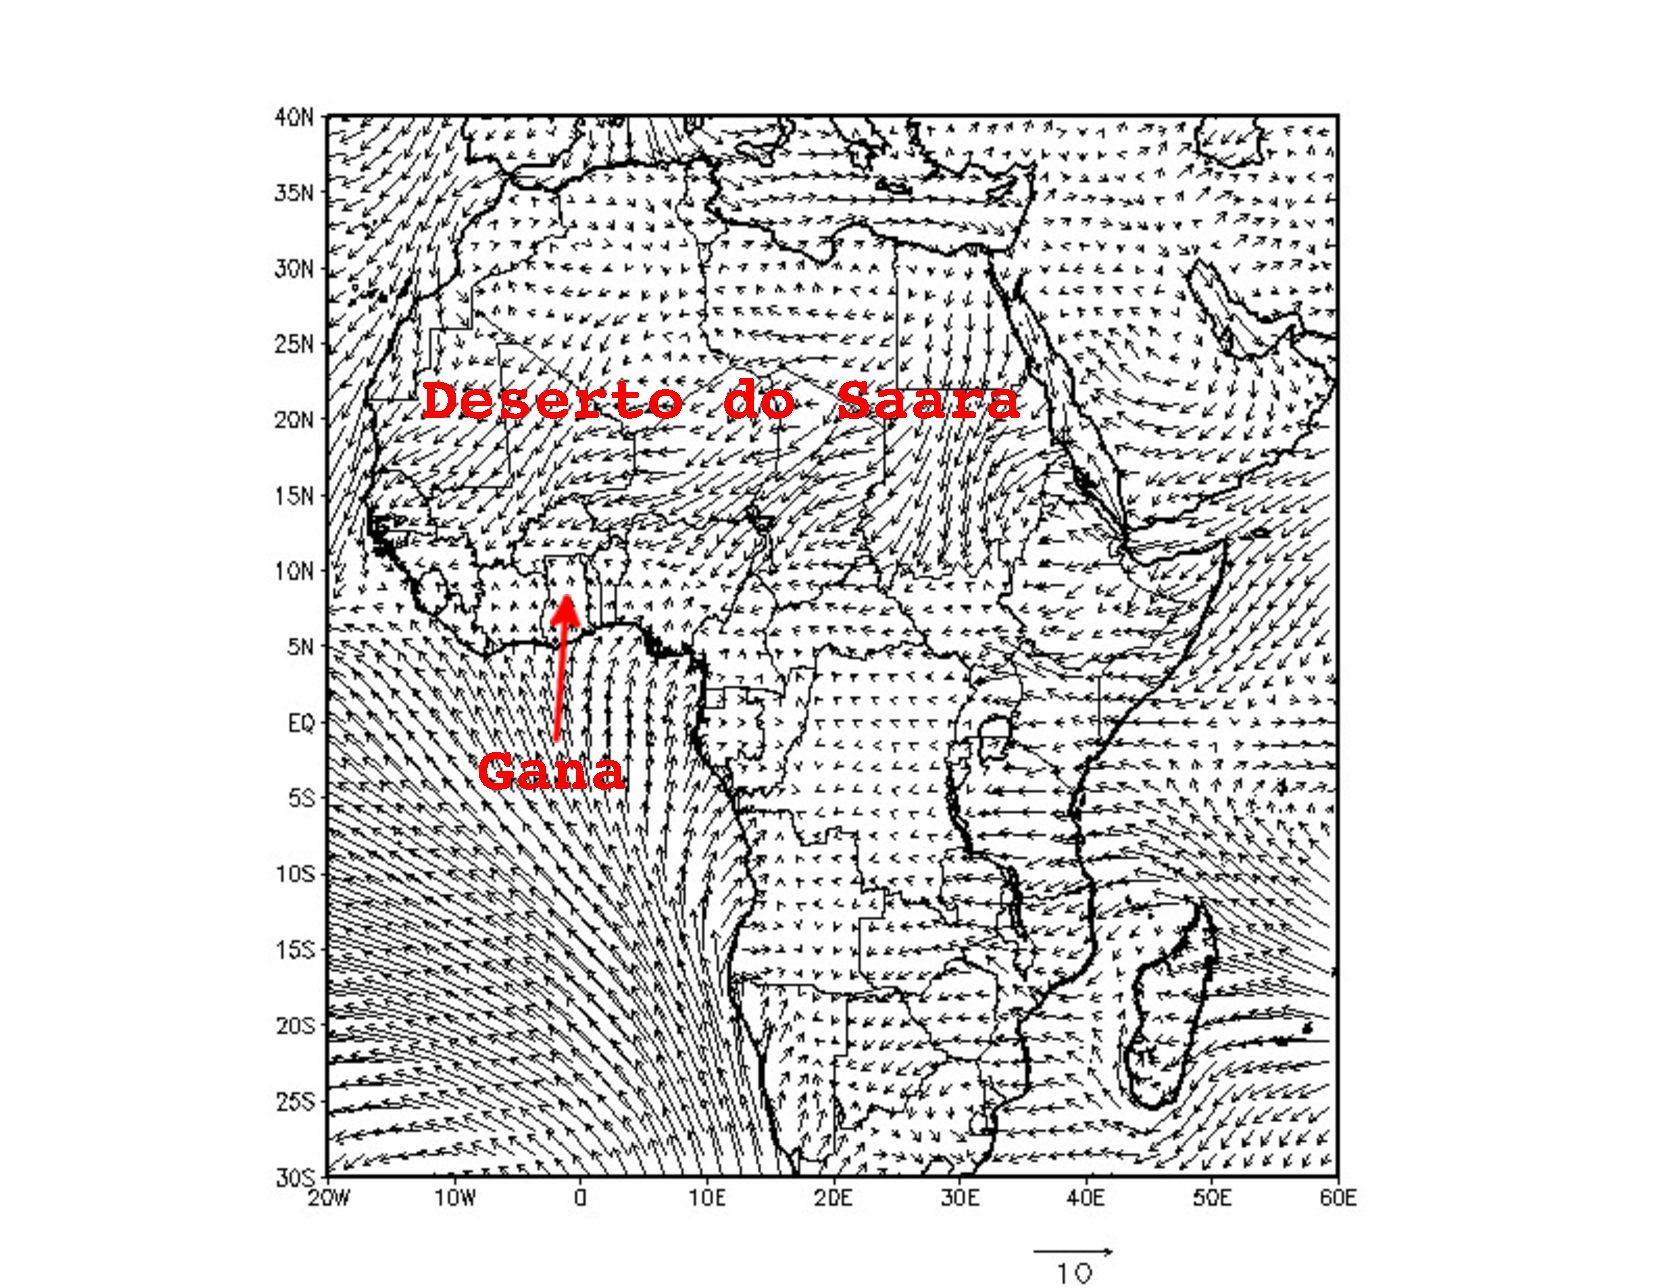
\includegraphics[width=\linewidth]{../inputs/grads/gimp/1000hPa/DEZ_2007.pdf}
    \caption{Dezembro de 2007}
  \end{subfigure}%
%  \hspace{0.5cm}
  \begin{subfigure}[b]{0.5\linewidth}
    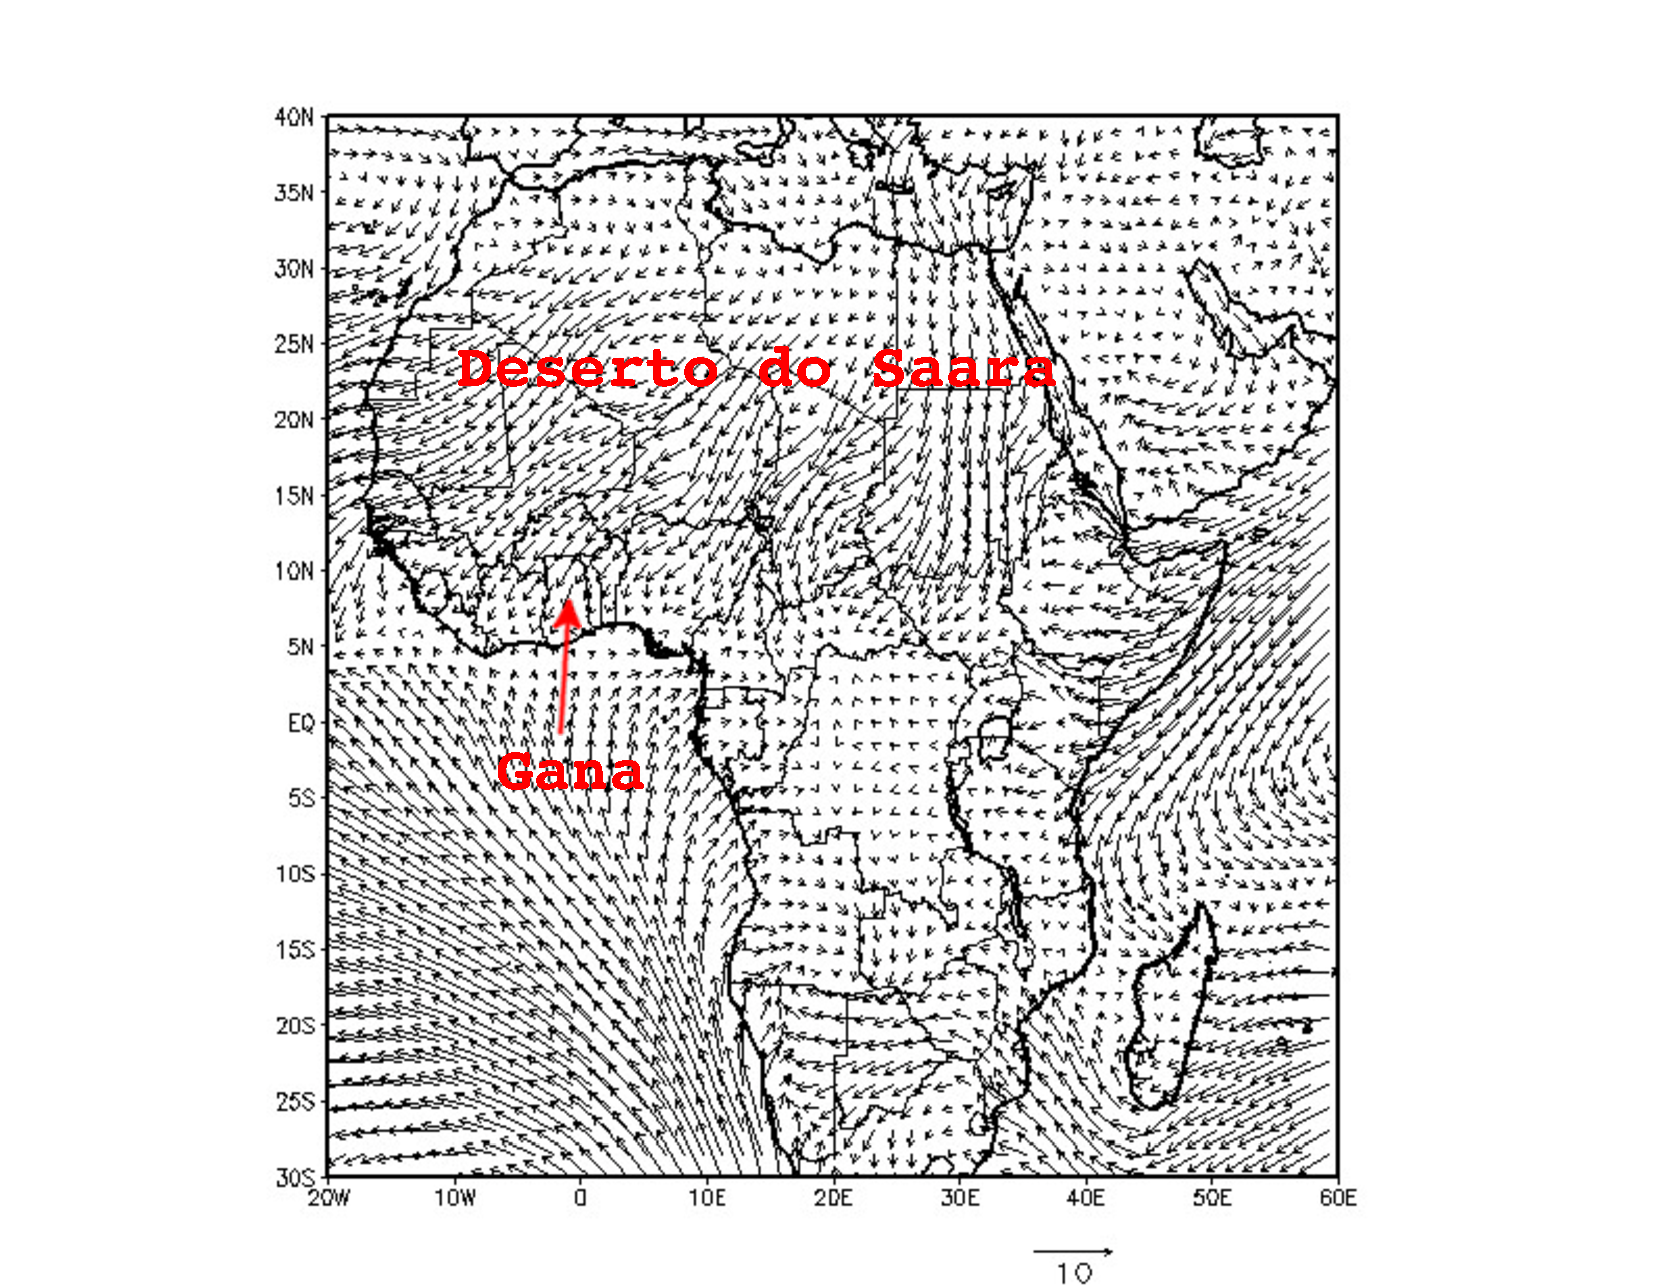
\includegraphics[width=\linewidth]{../inputs/grads/gimp/1000hPa/JAN_2008.pdf}
    \caption{Janeiro de 2008}
  \end{subfigure}
  \caption{Intensidade e direção do vento médio na superfície (10 metros) no 
           continente Africano. \label{fig:ECMWF10} }
\end{figure}


